\documentclass[11pt]{article}
\usepackage[margin=0.85in]{geometry}
\usepackage[T1]{fontenc}
\usepackage{amsmath,amssymb,graphicx,longtable,tabularx,natbib,hyperref}
\newcommand{\toprule}{\hline}
\newcommand{\midrule}{\hline}
\newcommand{\bottomrule}{\hline}
\newcolumntype{Y}{>{\raggedright\arraybackslash}X}
\renewcommand{\topfraction}{0.9}
\renewcommand{\bottomfraction}{0.9}
\renewcommand{\textfraction}{0.05}
\renewcommand{\floatpagefraction}{0.8}
\hypersetup{colorlinks=true,linkcolor=blue,citecolor=blue,urlcolor=blue}
\newcommand{\tg}{\mathrm{Tg\ CH_4\ yr^{-1}}}
\title{Reconstructing the methane surge with a 2019 reference budget}
\author{Reproducible research report}
\date{8 October 2026}
\begin{document}
\maketitle
\begin{abstract}
Methane growth reflects both changes in sources and sinks and continued
adjustment toward an existing equilibrium. We implement the annual budget
decomposition of He et al. in Python and examine the publicly accessible
2019--2022 results without performing a flux inversion. Digitized central
curves reconstruct their first two figures over the requested period;
published tables and archived fluxes support additional comparisons. The
2020 emission anomaly ranges from about 7 to 37 Tg CH$_4$ per year among the
available reconstructions. Using NOAA annual surface methane as a common
burden proxy, the additional removal caused by rising methane amounts to
3.4, 7.8, and 12.3 Tg yr$^{-1}$ in 2020--2022 for a 10-year chemical lifetime.
These corrections do not remove differences in the studies' 2019 reference
states or OH diagnostics. The archived Peng fluxes reproduce the published
2020 anomaly to within $10^{-6}$ Tg when integrated over calendar years;
normalizing both years to 365 days changes that anomaly by 1.53 Tg.
All nine listed papers and their supporting materials were reviewed. Qu
(2022) supplies a native burden-based OH forcing of 4.66 Tg yr$^{-1}$ from
rounded table entries. Ciais's headline OH fraction uses a different temporal
operator and cannot be compared directly with He's forcing fraction.
Exact posterior reproduction remains limited by the numerical output available.
\end{abstract}

\section{Scope and available evidence}
The target is the steady-state adjustment of \citet{heetal2026a}, not a new
estimate of methane fluxes from atmospheric observations. We use 2019 as the
reference in every anomaly calculation and retain 2019--2022. Absolute
baseline quantities appear only where needed to interpret the anomalies.
All nine bibliography entries were read in full: \citet{heetal2026a,
ciaisetal2026,fengetal2023,laughneretal2021,pengetal2022,quetal2022,
quetal2024,stevensonetal2022,lawrenceetal2001}. This includes their
supplementary PDFs, appendices, and numerical workbooks. Standalone one-page
reading notes are retained in \texttt{literature/}. Publisher access failures
were resolved with locally supplied Ciais and Qu (2022) articles and
supplements, and Laughner's four supplementary files. Their identities,
page counts, and checksums are recorded in \path{data/provided_sources.json}.
The original PDFs are retained locally; extracted numerical inputs and all
project code, notes, figures, and report sources are in the repository.

\section{Budget decomposition and scientific decisions}
Let $m_j$ denote annual representative atmospheric methane mass, $E_j$ gross
emissions, $L_j$ positive soil uptake, and $k_j=k_{\rm OH,j}+k_{\rm other,j}$
the chemical loss frequency. Mass is in Tg CH$_4$, fluxes in Tg CH$_4$
yr$^{-1}$, and loss frequencies in yr$^{-1}$. The annualized global budget is
\begin{equation}\label{eq:budget}
G_j=E_j-k_jm_j-L_j,
\end{equation}
in which $G_j$ is the atmospheric growth rate. A subscript 0 denotes 2019
and $\Delta x_j=x_j-x_0$ within each reconstruction. Expanding gives
\begin{equation}\label{eq:he}
G_j=\underbrace{G_0-k_0\Delta m_j}_{R_j}
 +\underbrace{\Delta E_j}_{F_{E,j}}
 \underbrace{-m_0\Delta k_{\rm OH,j}}_{F_{{\rm OH},j}}
 +\epsilon_j,
\end{equation}
\begin{equation}\label{eq:residual}
\epsilon_j=-m_0\Delta k_{\rm other,j}
 -\Delta k_j\Delta m_j-\Delta L_j.
\end{equation}
He neglects $\epsilon_j$. The code returns both this approximation and the
exact residual, allowing its validity to be checked when all inputs are
available. Soil uptake is not included a second time in $k_0$.
An increasing burden makes the relaxation contribution $R_j$ smaller even
when emissions and chemical loss frequencies are unchanged. In anomaly form,
\begin{equation}\label{eq:adjust}
\Delta G_j+k_0\Delta m_j\simeq F_{E,j}+F_{{\rm OH},j}.
\end{equation}
The adjustment has a positive sign on the left: growing methane increases
removal under the reference loss frequency. A growth-rate anomaly by itself
understates the forcing needed to sustain that growth.

\paragraph{Counterfactual definition.}
For constant $E_0,L_0,k_0$ and initial burden $m_c(0)=m_0$, the separately
integrated counterfactual is
\begin{equation}\label{eq:counter}
m_c(t)=m_0+(E_0-L_0-k_0m_0)\frac{1-e^{-k_0t}}{k_0}.
\end{equation}
This is an exact constant-parameter box-model solution. It evaluates losses
on $m_c(t)$; Eq.~\ref{eq:he} evaluates reference losses on the actual burden
$m_j$. These are distinct diagnostics when the actual and counterfactual
trajectories diverge. We implement both and do not equate their integrals.
The dashed curves in the reconstructed He figure are digitized published
curves, because the native initial burden and all reference losses are not
provided numerically in the acquired materials.

\paragraph{Hydroxyl radical (OH) sink definition.}
If a study supplies positive OH removal $Q_j=k_{\rm OH,j}m_j$, the equivalent
baseline-burden forcing is
\begin{equation}\label{eq:oh}
F_{{\rm OH},j}=Q_0-Q_j\frac{m_0}{m_j}.
\end{equation}
It is generally different from the raw removal saving $Q_0-Q_j$.
An area- or mass-weighted mean OH change cannot simply replace
$\Delta k_{\rm OH}$. \citet{lawrenceetal2001} show that averaging weights,
temperature, and the atmospheric domain change the relationship between mean
OH and oxidation. We therefore do not convert Feng's latitude-band OH
diagnostic or Qu's area-weighted supplementary OH curve directly to a flux.
Nor do we substitute a methane perturbation lifetime, which incorporates
chemical feedback, for He's chemical lifetime.

\paragraph{Common-burden sensitivity.}
For Qu (2024)'s tabulated OH removal, a native application of Eq.~\ref{eq:oh}
requires unavailable matched annual model burdens. We additionally evaluate
it with $m^*_j=2.77X_j$, in which $X_j$ is NOAA's global annual surface mean
in ppb and 2.77 Tg ppb$^{-1}$ follows He. This assumption is explicit: a
surface mean is a proxy for the whole-atmosphere burden. Its fractional
growth, rather than its constant multiplicative conversion, controls
Eq.~\ref{eq:oh}. The result is labeled ``common burden,'' not native Qu
forcing. Qu (2022), in contrast, tabulates its native burdens and does not
require this substitution. To evaluate Eq.~\ref{eq:adjust} for NOAA growth, we examine chemical
lifetimes of 9, 10, 11, and 12 years. This sensitivity range brackets the
roughly 11-year OH lifetimes reported by He and Qu while allowing additional
chemical losses; it is not a fitted or independently inferred lifetime.
Soil uptake and other chemical frequencies are held fixed in this diagnostic.

\paragraph{Signed removal changes and prescribed OH scenarios.}
Ciais Fig.~S3 supplies signed OH sink $S=-Q$ relative to 2010, but not
absolute 2019 removal or annual model burden. We subtract each series'
2019 value, $s_j=S_j-S_0$, so every plotted anomaly uses 2019. For an
assumed OH-only lifetime $\tau_{{\rm OH},0}$ and NOAA burden proxy,
\begin{equation}\label{eq:ciais}
F^*_{{\rm OH},j}=\frac{m^*_0}{m^*_j}
\left(s_j+\frac{m^*_j-m^*_0}{\tau_{{\rm OH},0}}\right).
\end{equation}
We use 11.1 yr as a benchmark, motivated by He's reported mean OH lifetime,
and test 9--12 yr. This does not establish Ciais's native 2019 lifetime.
The same benchmark translates a uniform prescribed OH reduction $r$ into
\begin{equation}\label{eq:uniform}
F^*_{{\rm OH},2020}=r\,m^*_0/\tau_{{\rm OH},0}.
\end{equation}
These calculations hold baseline weighting and temperature fixed and are
conditional comparisons, not recovered posterior results. The derivation is
retained in \path{docs/derivations/published_removal_anomalies.tex}.

\paragraph{Time and uncertainty.}
NOAA reports annual mean concentrations and growth from January to January.
These are different observables and are retained with their own labels.
The downloaded NOAA files were created in September 2026 and are not the
November 2025 snapshot cited by He. Annual mean burden approximates the
burden relevant to an annual budget; no subannual covariance is reconstructed.
The original NOAA annual-mean and growth files are archived with this project;
their public endpoints are
\href{https://gml.noaa.gov/webdata/ccgg/trends/ch4/ch4_annmean_gl.txt}{annual means}
and \href{https://gml.noaa.gov/webdata/ccgg/trends/ch4/ch4_gr_gl.txt}{annual growth}.
Missing years and missing sink components remain missing. We do not combine
annual posterior standard deviations into anomaly errors without their
cross-year covariance, and we do not invent common uncertainty intervals
for studies with different ensembles and uncertainty definitions.

\section{Reconstructing the He figures}
Figure~\ref{fig:he1} reconstructs the 2019--2022 portion of He's Fig.~1 from
the public raster and adds the current numerical NOAA record. The plotted
quantity is concentration change, despite the growth-rate wording in the
original title. Figure~\ref{fig:he2} reconstructs the central curves of all
four panels in He's Fig.~2, expressing emissions, lifetime, sectors, and
growth as anomalies from 2019. The original uncertainty envelopes are not
reproduced. Panel B subtracts the 2019 relaxation term, so the relaxation
anomaly is negative while the original absolute relaxation contribution
remains positive.

The file \path{data/he_digitization.json} records the selected pixels and
axis calibrations. A two-pixel coordinate
allowance corresponds to about 1.1 Tg yr$^{-1}$ for an individual total
emission value and 0.5 Tg yr$^{-1}$ for an individual stacked-bar boundary.
Differences between two selected points can have twice those worst-case
bounds. These are digitization tolerances, not posterior uncertainty.
The independently digitized emission changes in panels A and B agree to
within 0.35 Tg yr$^{-1}$. This checks transcription consistency, not the
validity of the inversion.

\begin{figure}[htbp]\centering
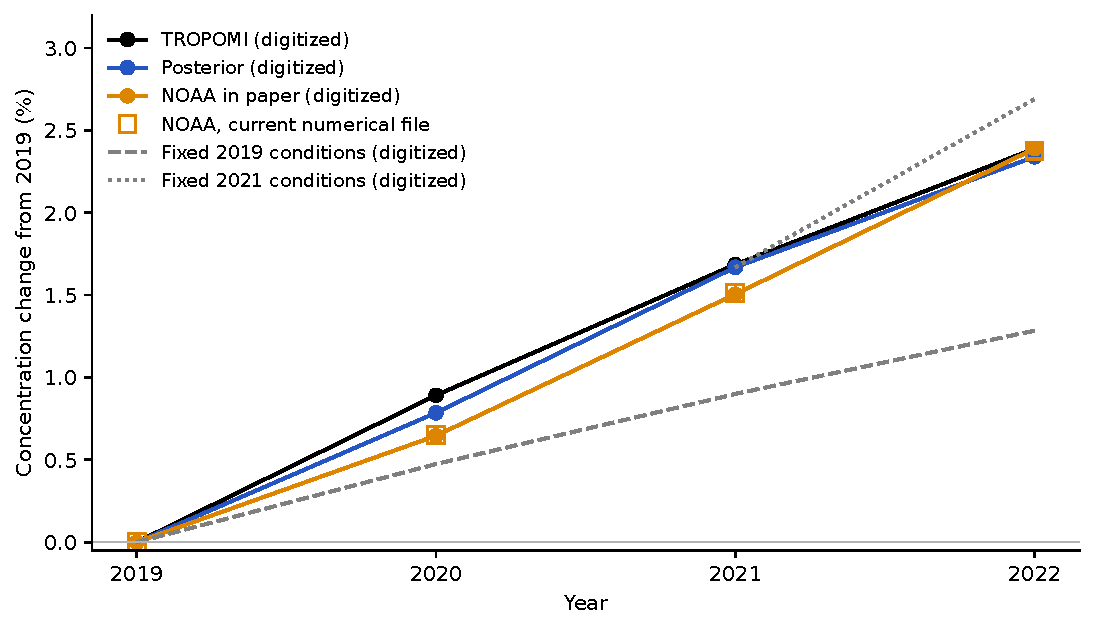
\includegraphics[width=.87\linewidth]{../figures/he_figure1.pdf}
\caption{Reconstruction of He Fig.~1 for 2019--2022. Black, blue, and orange
filled markers are digitized TROPOMI, posterior GEOS--Chem, and published NOAA
concentration changes, respectively. Orange open squares use the September
2026 NOAA numerical file. Gray dashed and dotted curves are the published
fixed-2019 and fixed-2021 counterfactuals, respectively, digitized without
refitting. All concentration changes are expressed as percentages of their own
2019 values. The fixed-2021 branch retains the same 2019 reference.}
\label{fig:he1}\end{figure}

\begin{figure}[htbp]\centering
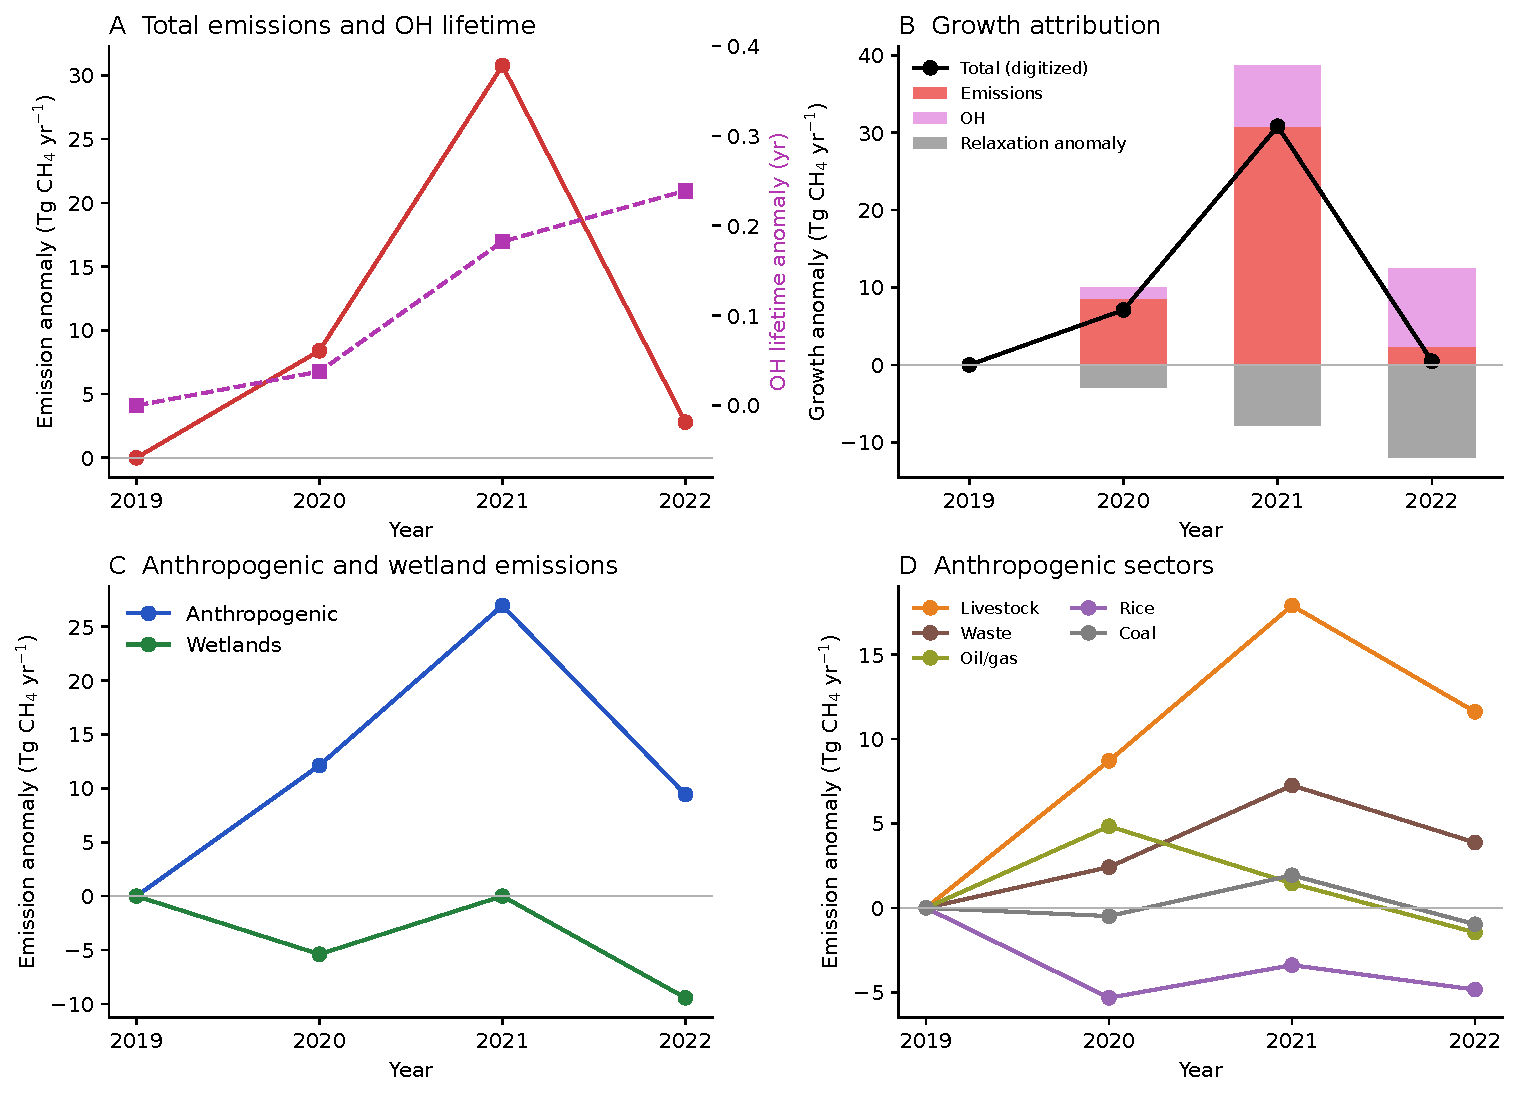
\includegraphics[width=\linewidth]{../figures/he_figure2.pdf}
\caption{Reconstruction of He Fig.~2 central values, rebased to 2019.
(A) Red emission changes and purple changes in lifetime against tropospheric
OH. (B) Red emission forcing, pink OH forcing, and gray relaxation anomalies;
the black curve is their sum. The original positive baseline relaxation is
subtracted. (C) Anthropogenic and wetland emission changes. (D) Changes in
the five displayed anthropogenic sectors. Curves are digitized; shaded
posterior ranges are omitted. Sector attribution inherits He's prior sector
fractions. The panels are not independent flux inversions.}
\label{fig:he2}\end{figure}

\section{Comparing emission and sink changes}
Table~\ref{tab:annual} and Fig.~\ref{fig:flux} show the available annual
global anomalies. The largest emission disagreement is in 2020: Qu (2024)'s
37 Tg yr$^{-1}$ exceeds digitized He by about 29 Tg yr$^{-1}$ and Feng's
joint-OH estimate by 19.1 Tg yr$^{-1}$. The He--Qu difference narrows to
about 9 Tg yr$^{-1}$ in 2021, then widens to about 16 Tg yr$^{-1}$ in 2022.
Qu (2022) gives 31 Tg yr$^{-1}$ in 2020, while Ciais reports
$22.0\pm3.5$ Tg yr$^{-1}$. The digitized Ciais central emission changes are
21.9, 24.9, and 23.4 Tg yr$^{-1}$ in 2020--2022. Thus Ciais and He also
differ by about 21 Tg yr$^{-1}$ in 2022. These comparisons preserve each
study's own 2019 emissions. They do not imply
that the reconstructions share the same absolute emission baseline.

\begin{table}[htbp]\centering\small
\begin{tabular}{lrrr}
\toprule Study / quantity & 2020 & 2021 & 2022 \\
\midrule
He emissions (digitized) & 8.4 & 30.8 & 2.8 \\
He OH forcing (digitized) & 1.5 & 7.8 & 10.0 \\
He relaxation anomaly (digitized) & -2.9 & -7.8 & -12.0 \\
Qu 2022 emissions & 31.0 & --- & --- \\
Qu 2022 OH forcing, native burden & 4.7 & --- & --- \\
Ciais emissions (digitized) & 21.9 & 24.9 & 23.4 \\
Ciais OH-1, conditional & 6.4 & 22.8 & 14.1 \\
Ciais OH-2, conditional & 7.3 & 15.3 & 10.1 \\
Qu 2024 emissions & 37.0 & 40.0 & 19.0 \\
Qu 2024 OH removal saving & 11.0 & 10.0 & 25.0 \\
Qu 2024 OH forcing, common burden & 14.0 & 17.0 & 35.5 \\
Feng emissions, joint OH & 17.9 & 18.4 & --- \\
Feng emissions, fixed OH & 27.0 & 20.8 & --- \\
NOAA growth anomaly & 14.2 & 22.3 & 9.3 \\
Burden adjustment, $\tau_0=10$ yr & 3.4 & 7.8 & 12.3 \\
\bottomrule
\end{tabular}

\caption{Annual anomalies relative to 2019 in Tg CH$_4$ yr$^{-1}$.
He and Ciais values are digitized central estimates. Qu (2022) uses rounded
Table 1; Qu (2024) uses Table S1; Feng uses Table 1. Qu (2022)'s OH forcing
uses native burden. Qu (2024)'s common-burden OH forcing
uses Eq.~\ref{eq:oh} and NOAA annual surface means. It is conditional, whereas
the raw removal saving is a direct table difference. Ciais OH-1 and OH-2 use
Eq.~\ref{eq:ciais} with an assumed 11.1-yr 2019 OH lifetime. The last row is a
sensitivity calculation, not another inversion. Dashes denote unavailable
years. All anomalies are zero in 2019 by definition.}
\label{tab:annual}\end{table}

\begin{figure}[htbp]\centering
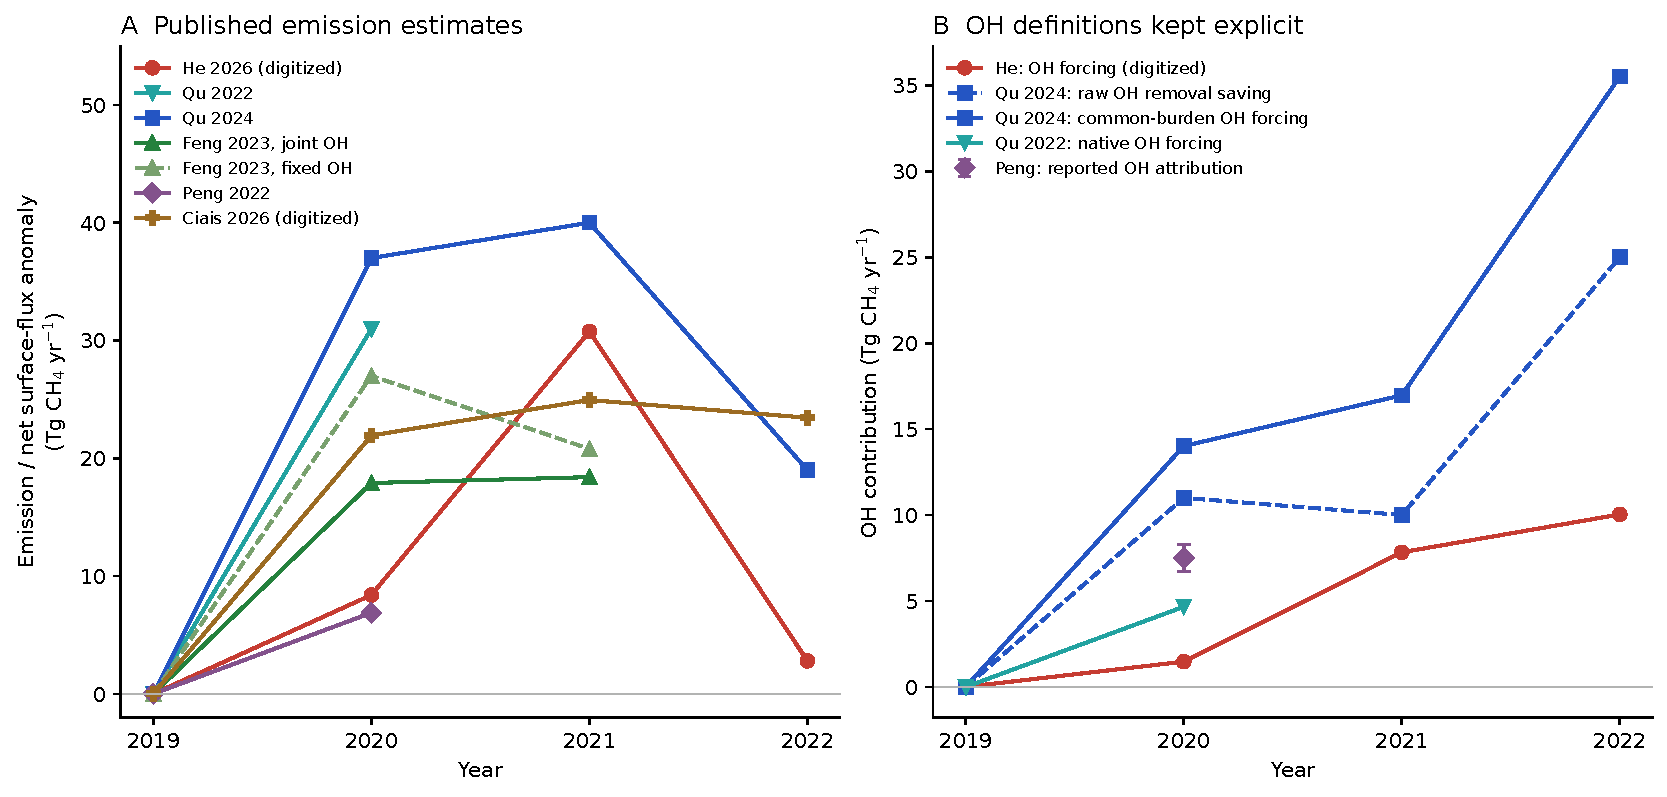
\includegraphics[width=\linewidth]{../figures/flux_comparison.pdf}
\caption{Global emission and OH comparisons. (A) Emission anomalies from
He (red), Qu 2024 (blue), Qu 2022 (teal), Ciais (brown), Feng joint and fixed
OH (green solid and dashed), and Peng (purple). Peng's calendar-year net surface-flux difference
is retained; the time-normalization distinction is quantified below.
(B) He OH forcing (red), Qu 2022 native forcing (teal), Qu 2024 raw OH removal
saving (blue dashed), and Qu 2024 common-burden forcing (blue solid). The purple
diamond and error bar are Peng's reported $7.5\pm0.8$ Tg yr$^{-1}$ OH
attribution; its definition is not silently replaced by the Qu diagnostic.
Lines end where each study's available period ends.}
\label{fig:flux}\end{figure}

\paragraph{The sink correction grows through 2022.}
For Qu (2024), raw OH removal savings of 11, 10, and 25 Tg yr$^{-1}$ become about
14, 17, and 36 Tg yr$^{-1}$ under the common-burden calculation.
This occurs because maintaining even the reduced removal flux at a larger
burden requires a larger decline in loss frequency than the raw flux change
suggests. At a 10-year chemical lifetime, the NOAA burden adjustment is
3.36, 7.81, and 12.29 Tg yr$^{-1}$. Varying the lifetime from 9 to 12 years
changes the 2022 correction from 13.65 to 10.24 Tg yr$^{-1}$. The correction
therefore matters increasingly after the initial surge, but it does not
uniquely identify emissions versus OH.

\paragraph{The baseline is a separate discrepancy.}
Qu (2024)'s Table S1 reports 2019 emissions of 550 Tg yr$^{-1}$ and total removal
of 553 Tg yr$^{-1}$, implying growth of $-3$ Tg yr$^{-1}$. The corresponding
NOAA growth in the current file is $+26.70$ Tg yr$^{-1}$; digitized He is
about $+27.7$ Tg yr$^{-1}$. Qu's 2020 native growth of 45 Tg yr$^{-1}$ thus
represents a 48 Tg yr$^{-1}$ anomaly, even though its absolute 2020 growth
is near NOAA's 40.94 Tg yr$^{-1}$. Replacing Qu's baseline with NOAA would
change the question and obscure this initialization issue. Qu adjusts its
initial concentration each year, while its continuous diagnostic run does
not impose those resets. He propagates the posterior state with a Kalman
approach. These documented choices are plausible contributors to the
baseline difference; the available global tables cannot isolate their
individual effects.
Qu (2022) gives growth of 28 and 59 Tg yr$^{-1}$, a 31 Tg yr$^{-1}$ anomaly,
versus 14.24 Tg yr$^{-1}$ in our NOAA record. Its annual initial states are
independently scaled by 0.97 and 1.01. This native budget difference must be
retained even though the initial burden and 2019 emissions are close to He's.
It is not corrected by replacing the tabulated model growth with NOAA.

\begin{figure}[htbp]\centering
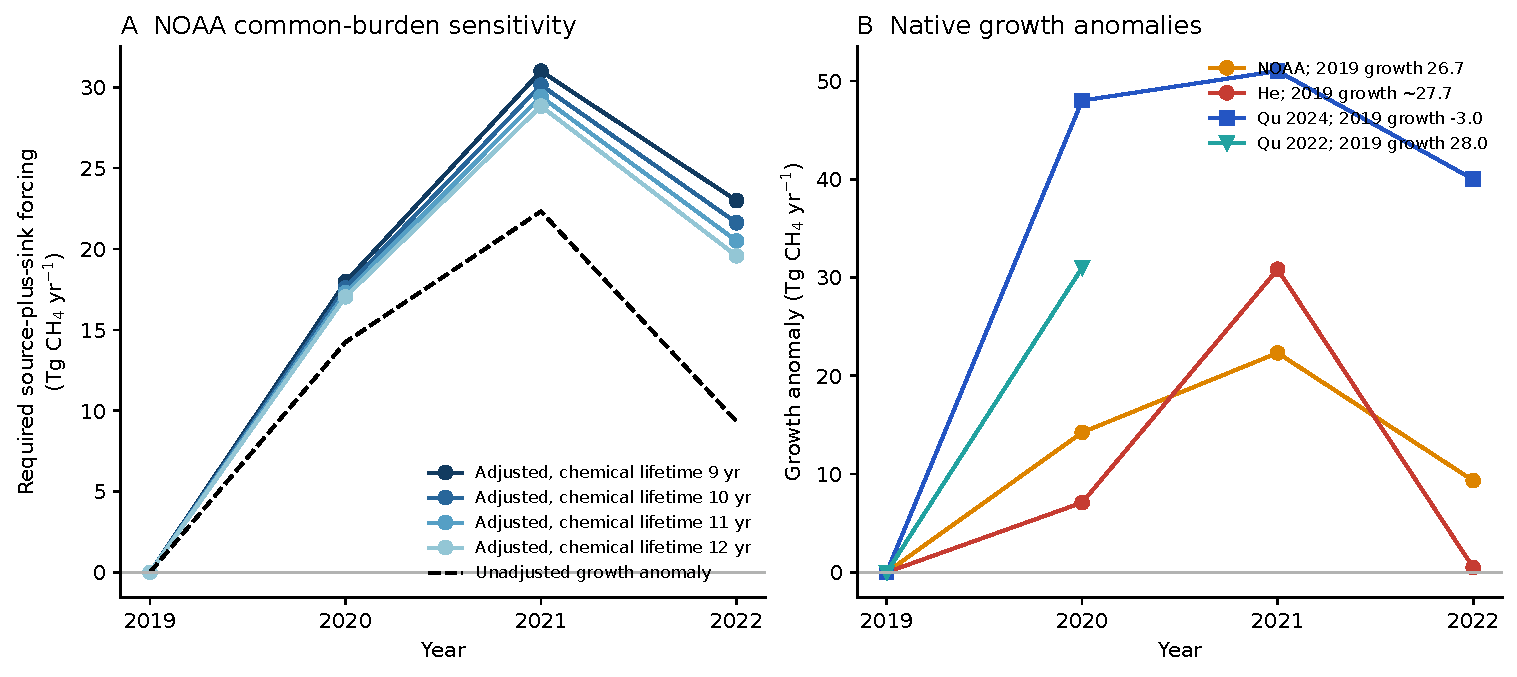
\includegraphics[width=\linewidth]{../figures/adjustment_and_baseline.pdf}
\caption{Adjustment sensitivity and native growth anomalies. (A) Blue
curves add $\Delta m/\tau_0$ to the current NOAA growth anomaly for chemical
lifetimes of 9--12 years; black dashed is unadjusted growth. (B) NOAA
(orange), digitized He (red), Qu 2024 (blue), and Qu 2022 (teal), each relative
to its own 2019 growth. Legend values state the absolute baseline growth in
Tg yr$^{-1}$. Annual mean surface methane is a burden proxy in A; the curves
are not calibrated to reproduce the posterior estimates in B.}
\label{fig:adjust}\end{figure}

\paragraph{Attribution fractions have different denominators.}
He reports 81\% emissions and 19\% OH for the additional forcing during
2020--2021; its 59/25/16\% relaxation/emissions/OH partition describes
2019--2024 total growth and is outside this report's period. Peng's 47/53\%
split concerns the 2020 growth-rate increase. Feng's 34\% OH contribution
in 2020 is inferred from the reduction in required emissions when OH is
optimized: the fixed-OH anomaly is 27.0 Tg yr$^{-1}$ and the joint-OH
anomaly is 17.9 Tg yr$^{-1}$. The 9.1 Tg yr$^{-1}$ difference is a useful
sensitivity result but is not itself a separately measured $-m_0\Delta k$.
Stevenson's $2.86\pm1.13$ ppb yr$^{-1}$ is a one-year response to precursor
changes, equivalent to $7.92\pm3.13$ Tg over a year using He's conversion.
We do not average these fractions into a consensus attribution.

\paragraph{Ciais's OH fraction answers a different question.}
The supplement of \citet{ciaisetal2026} defines its headline contribution as
\begin{equation}\label{eq:ciaisfraction}
\bar f_{\rm OH}=\frac{1}{4}\sum_{j=2020}^{2023}
\frac{S_j-S_{j-1}}{G_j-G_{j-1}},\qquad S_j=-Q_j.
\end{equation}
It averages fractions of adjacent-year growth changes, rather than ratios
of fixed-2019 source and OH forcings. The denominator can be small or change
sign, and 2023 lies outside the requested interval. The abstract reports
83\%; the main discussion gives 70--86\% for NOAA, whereas the conclusion
gives 74--80\%. We retain those distinctions and do not reinterpret the
headline percentage as variance explained or as $F_{\rm OH}/(F_E+F_{\rm OH})$.
The separately reported regression $R^2$ values are 0.5--0.7.

Figure~\ref{fig:ciais} instead uses annual inversion-mean removal circles
from Ciais Fig.~S3. Their raw 2019-based savings are approximately 3.4, 16.1,
and 3.4 Tg yr$^{-1}$ for OH-1, and 4.4, 8.5, and $-0.7$ for OH-2.
The conditional 11.1-yr correction gives 6.4, 22.8, and 14.1 for OH-1,
and 7.3, 15.3, and 10.1 for OH-2. The largest 2022 OH comparison remains
Qu (2024)'s 35.5 versus He's digitized 10.0 Tg yr$^{-1}$, although the former
depends on a substituted burden. Native Ciais closure cannot be checked
without the matching burden, growth diagnostic, and other losses.

\begin{figure}[htbp]\centering
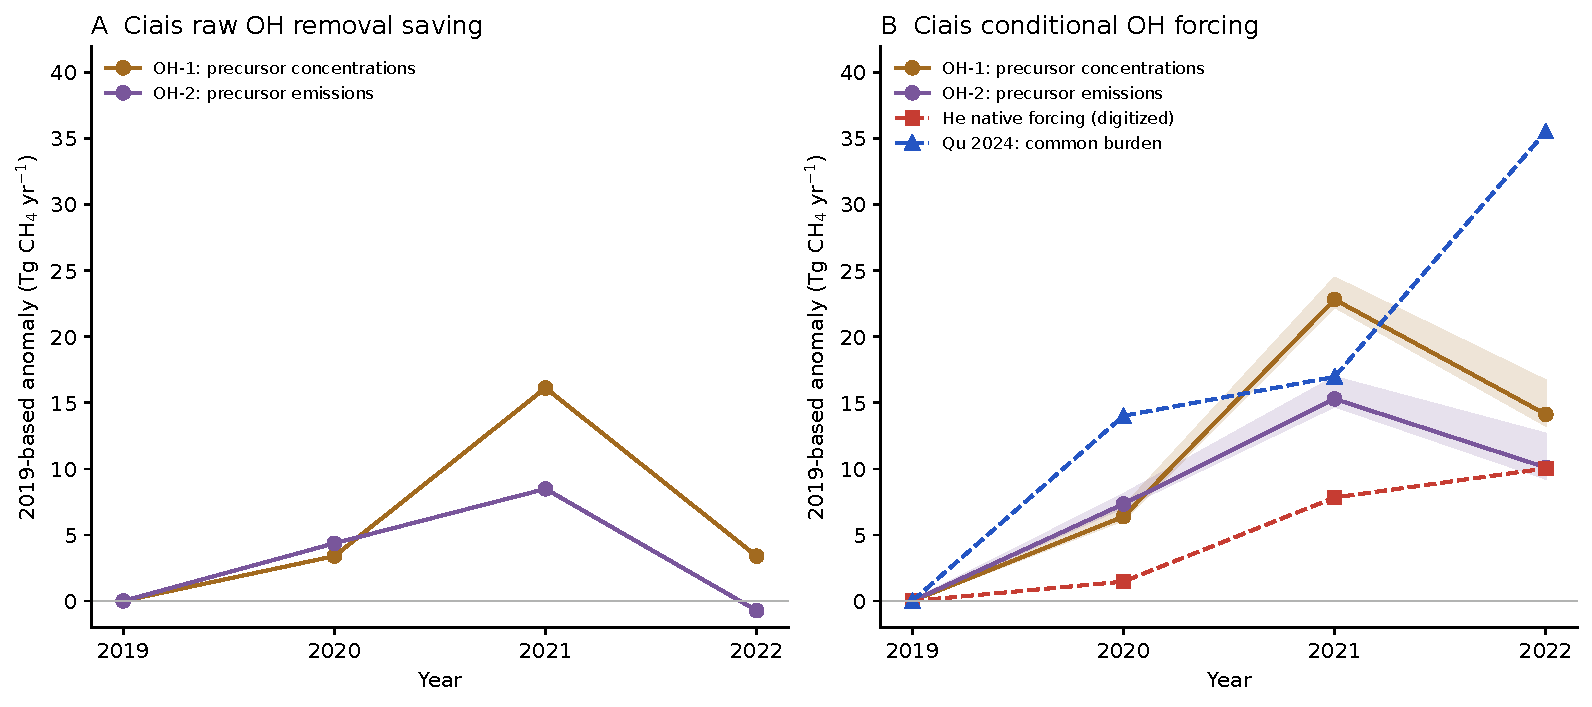
\includegraphics[width=\linewidth]{../figures/ciais_adjustment.pdf}
\caption{Ciais removal changes and the conditional steady-state adjustment.
(A) Brown and purple show OH-1 and OH-2 signed-removal changes after
subtracting 2019. (B) The same curves use Eq.~\ref{eq:ciais} with NOAA burden
and an assumed 11.1-yr OH lifetime; shading spans 9--12 yr and is not a
posterior uncertainty interval. Red dashed is He's digitized native OH
forcing; blue dashed is Qu (2024) with NOAA burden. Ciais's two-pixel reading
allowance implies a worst-case difference error of about 1 Tg yr$^{-1}$,
separate from both model spread and lifetime sensitivity. The published
2010 reference and the offset right axis are not used as anomaly baselines.}
\label{fig:ciais}\end{figure}

\paragraph{Laughner's scenario is now constrained by its supplement.}
\citet{laughneretal2021} prescribe a 3\% OH decrease during 2020 in a
two-hemisphere box model with the same emissions in perturbed and control
runs. Their 2--4\% range comes from March--May temporal variation in a
chemistry-assimilation experiment, not an annual posterior confidence
interval. Equation~\ref{eq:uniform} gives a conditional 2020 forcing of
14.0 Tg yr$^{-1}$ for 3\% and 11.1 yr, or 9.3--18.6 for 2--4\% at the same
lifetime. Jointly varying the lifetime over 9--12 yr broadens that range to
8.6--23.0. These are scenario equivalents, not new inferred fluxes.
The paper's plotted 2021 trajectories are explicitly extrapolated, not
box-model predictions. Its inventory workbook has no methane values for
2018--2020, so it cannot supply a 2019-baseline emission reconstruction.

\section{Why the reconstructions differ}
\begin{table}[htbp]\centering\small
\caption{Methods of all nine reviewed studies. These distinctions affect
source attribution, reference states, and sink meaning; they do not establish
a ranking or isolate the effect of each modeling choice.}\label{tab:methods}
\begin{tabularx}{\linewidth}{p{.10\linewidth}YYY}
\toprule Study & Observations and transport & Optimized or prescribed OH & Source and reference treatment\\
\midrule
He 2026 & TROPOMI; GEOS--Chem, $2^\circ\!\times2.5^\circ$; GEOS-FP & Two annual hemispheric factors; joint inversion & 4111 annual land fluxes; preceding posterior as prior; sectors from prior fractions\\
Qu 2022 & GOSAT land and glint; GEOS--Chem, $2^\circ\!\times2.5^\circ$; MERRA2 & One annual global OH loss-frequency factor; joint inversion & 4020 nonwetland and 168 wetland terms; independent annual priors and initial-state scaling\\
Qu 2024 & GOSAT including ocean glint; GEOS--Chem, $4^\circ\!\times5^\circ$; MERRA2 & Two annual hemispheric factors; joint inversion & Annual fixed prior; 1009 nonwetland grid fluxes and 168 monthly wetland terms; yearly initial-state scaling\\
Ciais 2026 & GOSAT; PYVAR--LMDz, WESTLAKE, and GONGGA, with different resolutions and assimilation windows & Prescribed precursor-concentration (OH-1) or emission-driven (OH-2) chemistry & Flat wetland priors; six model/OH combinations; mixed-cell source changes reallocated using bottom-up fractions\\
Feng 2023 & GOSAT CH$_4$/CO$_2$ ratios and surface constraints; GEOS--Chem, $2^\circ\!\times2.5^\circ$; MERRA2 & Fixed climatology or monthly factors in six latitude bands & Ensemble Kalman filter; 487 regions; four-month lag; regional fluxes\\
Peng 2022 & 103 surface sites; LMDZ--SACS, $1.9^\circ\!\times3.75^\circ$; ERA5 & Prescribed LMDZ--INCA chemistry; independent halocarbon check & Eight-day gridded net flux; variational inversion; bottom-up source attribution\\
Stevenson 2022 & HTAP chemistry response experiments, with 2020 precursor changes & Chemistry sensitivities and perturbation lifetimes & No methane flux inversion; 2001 sensitivities transferred to a 2020 pulse\\
Laughner 2021 & Two TCCON sites; two-hemisphere methane box model & Prescribed 3\% reduction during 2020, bracketed by 2--4\% & Same stabilized emissions in control and perturbation; observations referenced to a 2016--2019 trend\\
Lawrence 2001 & Four three-dimensional OH fields; global oxidation diagnostics & Compares averaging weights and atmospheric domains & Methodological study; no 2019--2022 reconstruction\\
\bottomrule
\end{tabularx}\end{table}

\paragraph{Tropical wetlands versus livestock.}
Qu (2024) assigns 43\% of its emission surge to Equatorial Asia and 30\% to Africa;
Feng's fixed-OH inversion gives a 2020 East African increase of
$14\pm3$ Tg relative to 2019. He finds a strong 2021 increase but assigns
much of its global source change to anthropogenic emissions, with wetlands
approximately unchanged from 2019 to 2021. This attribution depends on the
prior spatial overlap of livestock and wetlands: He optimizes their total
grid-cell flux and divides it using prior sector fractions, while Qu
optimizes monthly regional wetland fluxes separately. He's precipitation-driven
wetland prior can miss inundation displaced downstream from rainfall. Its
independent ammonia comparison does not support increased African livestock
emissions. Thus a livestock label in the posterior is not a direct
observation of a livestock increase.
Ciais applies a different additional assumption: in mixed cells, source
changes are reallocated when their agricultural fraction differs by more than
20\% from the corresponding bottom-up fraction. Its unmodified
prior-proportional allocation would assign $46.8\pm14.8$\% to agriculture
and waste and $34.7\pm4.6$\% to wetlands. Its wetland attribution is therefore
not a direct observation either. Ciais's air-mass-weighted OH maps and
isotope-box source tests constrain different aspects of the budget; neither
provides a replacement for annual reaction-weighted $k_{\rm OH}$.

\paragraph{South America and the baseline interval.}
Feng finds positive 2020 tropical South American emission changes and larger
2021 tropical and temperate South American increases. Qu (2024) emphasizes that
much of its South American increase preceded 2020, so it contributes less
to the 2020--2022 surge relative to 2019. He reports 2019--2024 trends, a
different endpoint interval that cannot be relabeled as 2019--2022. Without
common regional posterior arrays, a difference map or a precise regional
ranking across these reconstructions would imply information that is not
available. The global 2020 emission and 2022 OH differences are quantified;
regional explanations remain method-based comparisons.
Qu (2022) reports a 2020 South American total-emission reduction of
2.7 Tg yr$^{-1}$. Ciais reports a 2020--2022 mean reduction of
$1.4\pm0.8$ Tg yr$^{-1}$ specifically for southern South American wetlands,
with a north--south contrast within Amazonia. Those differences in sector,
boundary, and averaging interval preclude treating the two numbers as the
same regional observable. Across studies, Africa is a more consistent
location of increases than South America, but livestock versus inundated
wetland attribution remains sensitive to prior structure.

\paragraph{Chemistry and sampling.}
Peng prescribes three-dimensional OH changes simulated from changes in
precursor emissions and meteorology, while He, Qu, and Feng infer low-dimensional
OH factors from methane observations. The inferred split depends on prior
errors, transport, the spatial sampling of surface versus column observations,
and which OH degrees of freedom are allowed. Stevenson shows why a NO$_x$
reduction alone is insufficient: its positive 4.75 ppb yr$^{-1}$ contribution
is partly offset by negative CO and NMVOC contributions totaling about
1.90 ppb yr$^{-1}$. Applying a single OH percentage everywhere would conceal
this spatial and chemical structure.

\paragraph{A measured sensitivity of the inversion design.}
The nine cases in Qu (2022)'s main text and Table~S1 give a particularly
direct comparison (Fig.~\ref{fig:quensemble}). Reducing regularization from
the base 0.5 to 0.1 shifts the rounded source/OH forcing from 31/5 to 19/20
Tg yr$^{-1}$; increasing it to 1 gives 34/1. Changing only the OH prior
standard deviation from 5\% to 20\% leaves rounded emission forcing at
31 Tg yr$^{-1}$. Thus sensitivity cannot be judged from the OH prior alone.
The forcing stays within 35--39 across all cases, while the source--sink
split varies substantially. These are alternative inversion settings, not
independent posterior samples. They demonstrate a mechanism for attribution
differences without proving which setting explains the difference from He.

\begin{figure}[htbp]\centering
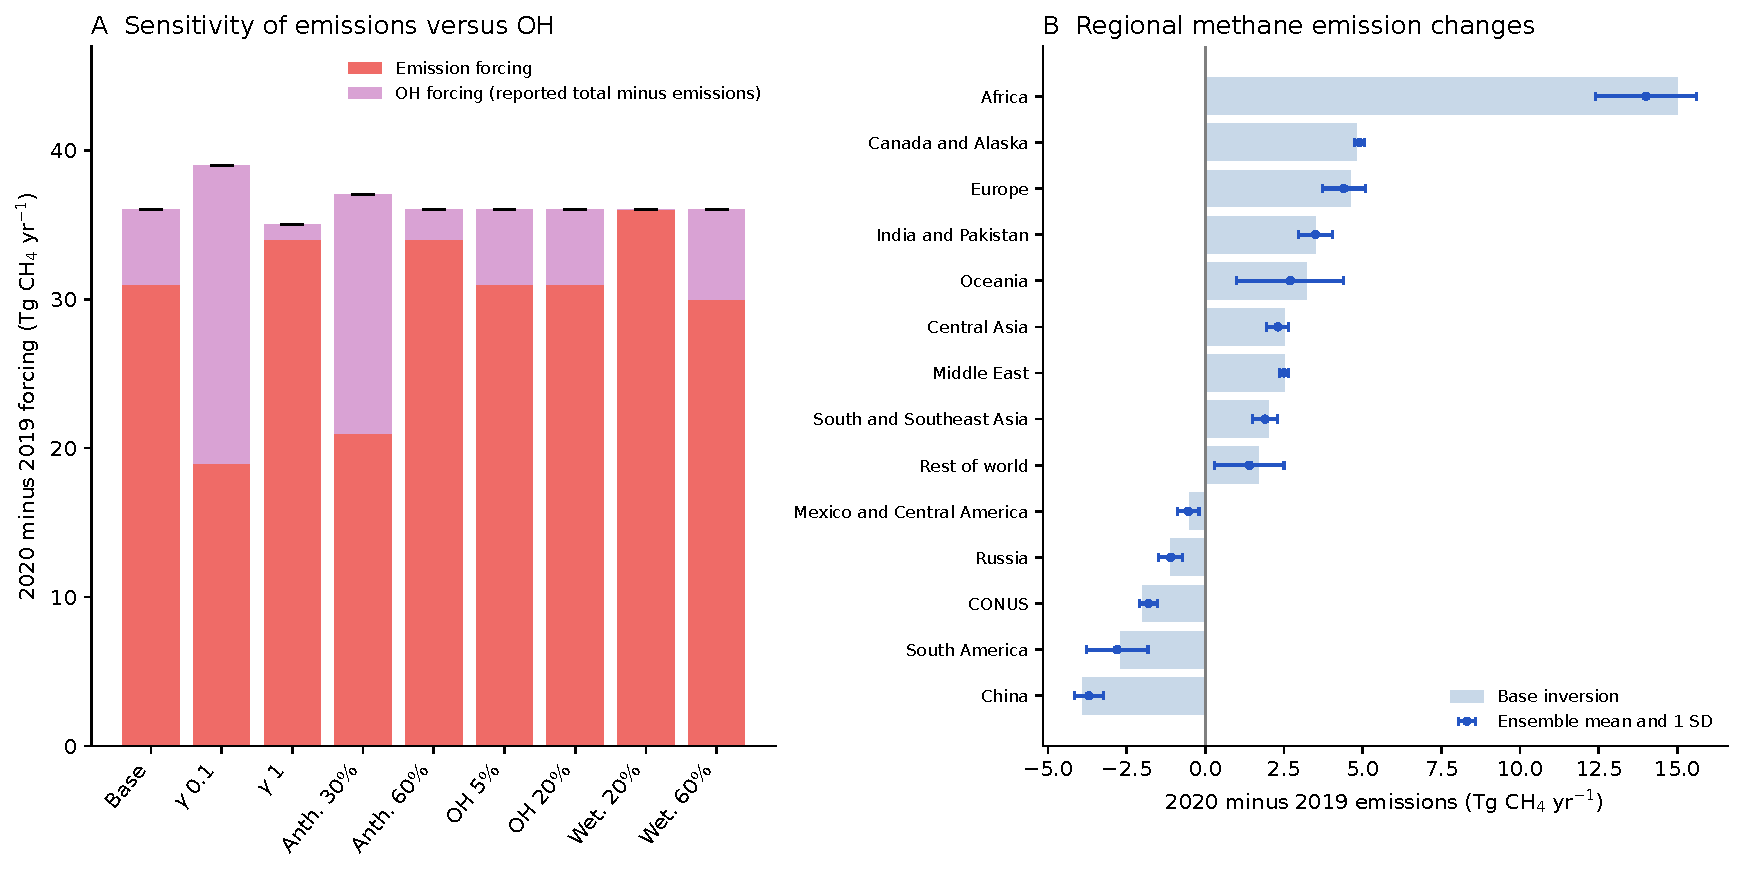
\includegraphics[width=\linewidth]{../figures/qu2022_sensitivity.pdf}
\caption{Qu (2022) sensitivity and regional evidence, all comparing 2020 with
2019. (A) Red bars are emission forcing; pink is reported total forcing minus
emissions, using rounded main-text and Table~S1 values. Black marks give total
forcing. Case labels identify regularization or the prior error standard
deviation changed from the base case. (B) Light-blue bars are Table~2 base
regional emission anomalies; dark-blue points and error bars are the reported
ensemble means and one-standard-deviation spreads. These regions do not match
Peng's latitude bands and are not silently aggregated into the same mask.
The figures are recalculations from published tables, not a repeated inversion.}
\label{fig:quensemble}\end{figure}

\begin{figure}[htbp]\centering
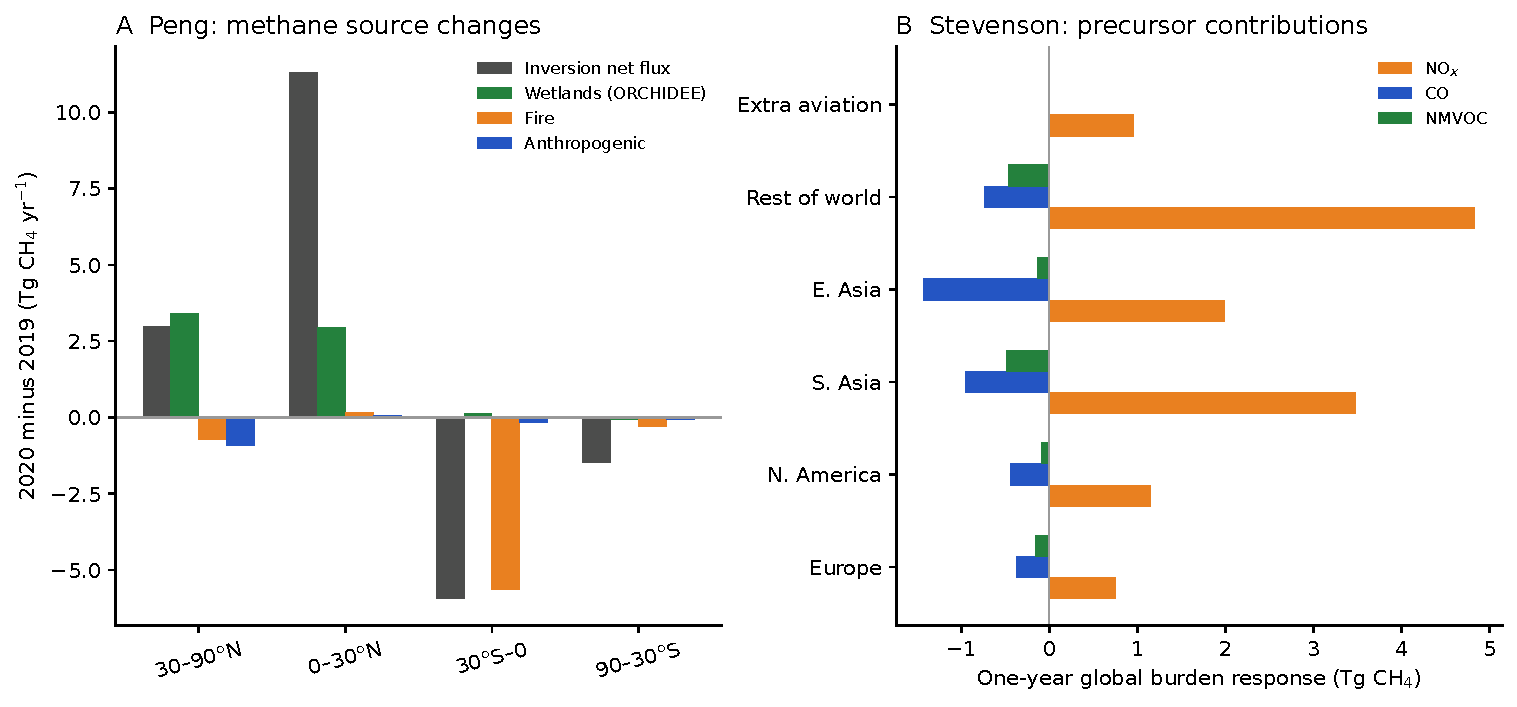
\includegraphics[width=\linewidth]{../figures/regional_evidence.pdf}
\caption{Regional evidence with distinct physical meanings. (A) Peng source
spreadsheet: 2020 minus 2019 methane inversion flux (gray), ORCHIDEE wetlands
(green), fire (orange), and anthropogenic sources (blue) in four latitude
bands. The bottom-up categories need not sum to the inversion. (B) Stevenson
Table S13a: global one-year methane burden responses to NO$_x$ (orange), CO
(blue), and NMVOC (green) emission changes in each source region, converted
with 2.77 Tg ppb$^{-1}$. Aviation is only the additional correction, avoiding
double counting. Panel B is not a map of regional methane emission changes.}
\label{fig:regional}\end{figure}

\section{A numerical reproduction of the Peng flux anomaly}
Peng's public monthly posterior is supplied in kg CH$_4$ m$^{-2}$ s$^{-1}$
with grid-cell areas in
\href{https://doi.org/10.6084/m9.figshare.21076171}{Figshare record 21076171}.
We multiply by area and the number of seconds in each
calendar month before summing. The reconstructed calendar-year totals are
552.5443 Tg in 2019 and 559.4283 Tg in 2020, giving 6.88403165 Tg. The
publisher spreadsheet gives 6.8840322 Tg, agreeing within $10^{-6}$ Tg.
This is a reproduction from numerical output, independent of figure digitization.

The same monthly data give mean rates of 552.5443 and 557.8998 Tg per 365-day
year. Their difference is 5.35554 Tg yr$^{-1}$; the extra 2020 day accounts
for 1.52849 Tg of the calendar-total difference. Both quantities are valid
when named correctly, but their units and temporal operators differ. We
retain the reported calendar total in the comparison and expose the alternative
rate normalization. This difference is smaller than the He--Qu emission gap
but comparable to some reported source changes. For the map in
Fig.~\ref{fig:pengmap}, we compare day-weighted annual mean rates, thereby
removing the purely calendar-length contribution.

\begin{figure}[htbp]\centering
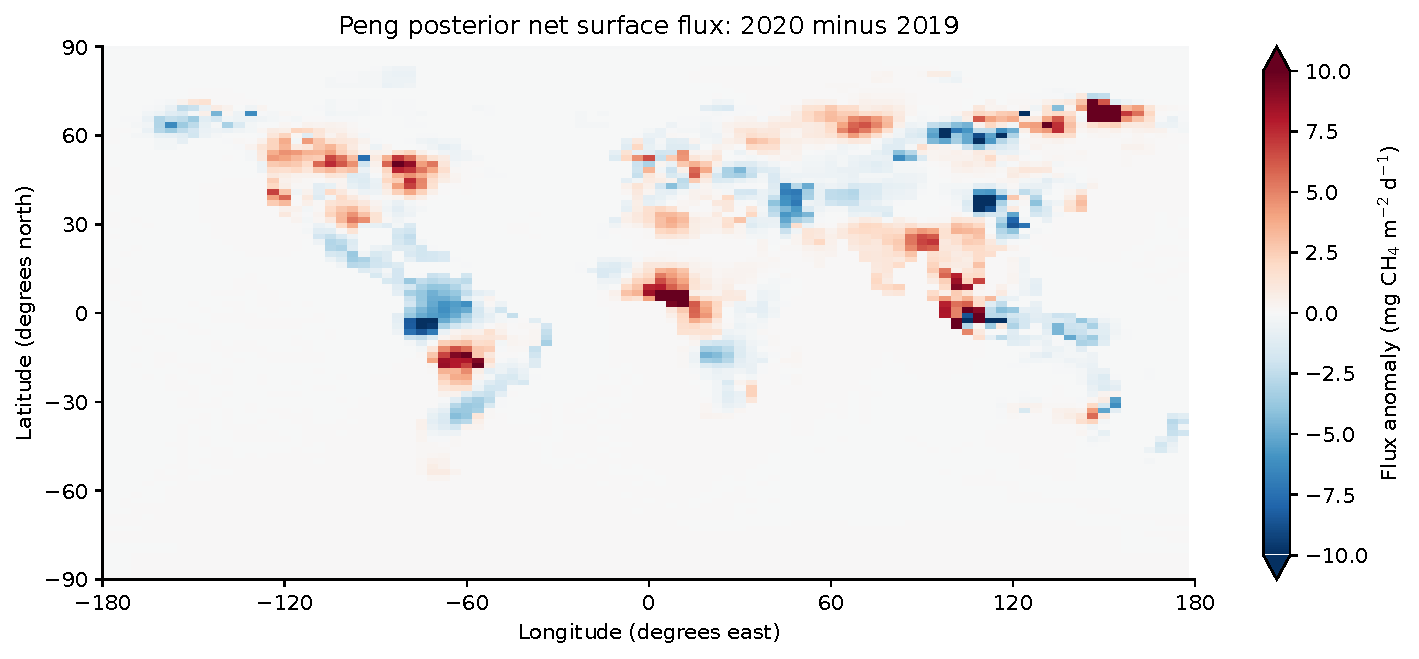
\includegraphics[width=\linewidth]{../figures/peng_flux_map.pdf}
\caption{Peng archived posterior net surface-flux rate, 2020 minus 2019.
Each annual field is weighted by days per month; colors show mg CH$_4$
m$^{-2}$ d$^{-1}$ with saturation at $\pm10$. Coordinates and grid-cell
areas come from the archived netCDF. Negative values are reductions relative
to 2019. This is a map of net surface flux, including prescribed soil uptake,
not a sector-resolved or regional OH attribution.}
\label{fig:pengmap}\end{figure}

\section{Reproducibility and remaining numerical limits}
\begin{longtable}{p{.17\linewidth}p{.76\linewidth}}
\toprule He figure & Reproduction status and required missing information\\\midrule
\endhead
1 & Central 2019--2022 curves digitized; updated NOAA numerical comparison
added. Native model mass, complete loss terms, and original NOAA snapshot
are needed for an exact independent counterfactual reproduction.\\
2A--D & Central time series digitized and rebased. Original ensemble members
and annual posterior diagnostics are needed for numerical curves and uncertainty
envelopes. No posterior inversion was performed.\\
3A--B & Not reconstructed. The map/pie and regional trends use 2024 or
2019--2024 endpoints and require gridded posterior sector data. They cannot
be converted to the target interval from the published image alone.\\
S1 & Fit maps and annual fit statistics require sampled prior/posterior
concentrations and observation-error diagnostics.\\
S2 & Averaging kernels and degrees of freedom require posterior covariance
and sensitivity matrices.\\
S3 & Sector trend maps require annual gridded sector fluxes; the published
2019--2024 trends cannot determine 2019--2022 anomalies.\\
S4 & The ammonia trend diagnostic covers 2019--2024 and requires the matched
IASI retrieval processing and regional masks. It is not a methane flux series.\\
S5 & The 2024 error-correlation matrix requires posterior covariance.\\
S6 & Prior wetland/anthropogenic overlap requires the actual gridded prior
files and masks used by the inversion; model code alone is insufficient.\\
S7 & TROPOMI/Carbon-I information-content experiment requires the specified
sensitivity and observation-error matrices; rebuilding it would require work
beyond the requested steady-state analysis.\\
S8 & The error-versus-observation-count diagnostic requires individual
2024 residuals and sampling information.\\
S9 & Comparison of regularization choices requires both posterior inversion
outputs. Re-running those inversions is explicitly out of scope.\\
\bottomrule
\end{longtable}

The public He availability statement points to model code and observational
inputs, rather than a numerical posterior archive sufficient for the items
above. Absence from those acquired materials is not proof that the authors
cannot provide the outputs. Complete annual burden, chemical loss, soil,
sector flux, and ensemble data would permit a native application of
Eq.~\ref{eq:he} and much stronger cross-study comparisons. We have not
substituted digitized diagnostic matrices or invented spatial flux fields.

The Python analysis, pinned pixi environment, original starter instructions,
download manifest with checksums, transcription tables, digitization
coordinates, processed netCDF files, executed figure notebook, reading notes,
and LaTeX sources are retained in the project repository. Four reusable budget tests check
algebraic closure, the constant-rate limit, analytical trajectories, and
baseline handling. Native full budgets remain unavailable, so these tests
validate the implementation rather than posterior numerical agreement.

All requested literature is now present and reviewed. Qu (2022)'s main and
supplementary budget tables, Ciais's bottom-up Table~S1 and digitized annual
markers, and Laughner's complete workbooks are retained as numerical inputs.
The Qu (2022) availability DOI points to GOSAT retrievals; the Ciais statement
points to the article and supplement. Neither supplies the full matched
posterior budget needed to reproduce all of He's terms for every study.
Ciais's other-natural-source treatment is described inconsistently on
supplement pp.~4--5 and in the main Fig.~2 caption; no unsupported component
is assigned from that ambiguity. Downloading a later inversion product would
not make it the posterior used in these papers.

The project reproduces the accessible numerical comparisons and clearly
labels graphical extraction and sensitivity calculations. Exact spatial,
ensemble, and counterfactual reconstruction of the remaining He figures
requires the author's numerical outputs, rather than a new inversion.

\bibliographystyle{plainnat}
\bibliography{references}
\end{document}
